
% Template for Elsevier CRC journal article
% version 1.2 dated 09 May 2011

% This file (c) 2009-2011 Elsevier Ltd.  Modifications may be freely made,
% provided the edited file is saved under a different name

% This file contains modifications for Procedia Engineering

% Changes since version 1.1
% - added "procedia" option compliant with ecrc.sty version 1.2a
%   (makes the layout approximately the same as the Word CRC template)
% - added example for generating copyright line in abstract

%-----------------------------------------------------------------------------------

%% This template uses the elsarticle.cls document class and the extension package ecrc.sty
%% For full documentation on usage of elsarticle.cls, consult the documentation "elsdoc.pdf"
%% Further resources available at http://www.elsevier.com/latex

%-----------------------------------------------------------------------------------

%%%%%%%%%%%%%%%%%%%%%%%%%%%%%%%%%%%%%%%%%%%%%%%%%%%%%%%%%%%%%%
%%%%%%%%%%%%%%%%%%%%%%%%%%%%%%%%%%%%%%%%%%%%%%%%%%%%%%%%%%%%%%
%%                                                          %%
%% Important note on usage                                  %%
%% -----------------------                                  %%
%% This file should normally be compiled with PDFLaTeX      %%
%% Using standard LaTeX should work but may produce clashes %%
%%                                                          %%
%%%%%%%%%%%%%%%%%%%%%%%%%%%%%%%%%%%%%%%%%%%%%%%%%%%%%%%%%%%%%%
%%%%%%%%%%%%%%%%%%%%%%%%%%%%%%%%%%%%%%%%%%%%%%%%%%%%%%%%%%%%%%

%% The '3p' and 'times' class options of elsarticle are used for Elsevier CRC
%% The 'procedia' option causes ecrc to approximate to the Word template
\documentclass[3p,times,procedia,number]{elsarticle}
\flushbottom

%% The `ecrc' package must be called to make the CRC functionality available
\usepackage{ecrc}
%\usepackage{amsmath}
\usepackage{amsmath}
\usepackage{amssymb}
\usepackage{bm}
%\usepackage[fleqn]{amsmath}
\usepackage{caption}
\usepackage{ulem}
\usepackage[colorlinks,linkcolor=blue,citecolor=blue,urlcolor=blue]{hyperref}
\usepackage{graphicx} 
\setcounter{totalnumber}{4}
\renewcommand{\textfraction}{0.15}
\renewcommand{\topfraction}{0.85}
\renewcommand{\bottomfraction}{0.65}
\renewcommand{\floatpagefraction}{0.60}
\newcommand{\figref}[1]{\figurename~\ref{#1}}
\usepackage{titlesec}
\titleformat{\chapter}[display]
{\normalfont\Large\bfseries}{\thechapter}{11pt}{\Large}
\titleformat{\section}
{\normalfont\large\bfseries}{\thesection}{11pt}{\large}
\titlespacing*{\chapter}{0pt}{0pt}{15pt} %left, beforesep, aftersep, right
\titlespacing*{\section}{0pt}{3.5ex plus 1ex minus .2ex}{2.3ex plus .2ex}
\usepackage[titletoc]{appendix}
\usepackage{listings}
\makeatletter
\newcommand{\rmnum}[1]{\romannumeral #1}
\newcommand{\Rmnum}[1]{\expandafter\@slowromancap\romannumeral #1@}
\makeatother
\newcommand{\HRule}{\rule{\linewidth}{0.5mm}}
\usepackage{xltxtra}

\usepackage[table,xcdraw]{xcolor}
\usepackage{datetime}
%% The ecrc package defines commands needed for running heads and logos.
%% For running heads, you can set the journal name, the volume, the starting page and the authors

%% set the volume if you know. Otherwise `00'
\volume{00}

%% set the starting page if not 1
\firstpage{1}

%% Give the name of the journal
\journalname{Procedia Engineering}

%% Give the author list to appear in the running head
%% Example \runauth{C.V. Radhakrishnan et al.}
\runauth{Ma Zepeng et al.}

%% The choice of journal logo is determined by the \jid and \jnltitlelogo commands.
%% A user-supplied logo with the name <\jid>logo.pdf will be inserted if present.
%% e.g. if \jid{yspmi} the system will look for a file yspmilogo.pdf
%% Otherwise the content of \jnltitlelogo will be set between horizontal lines as a default logo

%% Give the abbreviation of the Journal.
\jid{proeng}

%% Give a short journal name for the dummy logo (if needed)
%\jnltitlelogo{Procedia Engineering}

%% Hereafter the template follows `elsarticle'.
%% For more details see the existing template files elsarticle-template-harv.tex and elsarticle-template-num.tex.

%% Elsevier CRC generally uses a numbered reference style
%% For this, the conventions of elsarticle-template-num.tex should be followed (included below)
%% If using BibTeX, use the style file elsarticle-num.bst

%% End of ecrc-specific commands
%%%%%%%%%%%%%%%%%%%%%%%%%%%%%%%%%%%%%%%%%%%%%%%%%%%%%%%%%%%%%%%%%%%%%%%%%%

%% The amssymb package provides various useful mathematical syméls

\usepackage{amssymb}
%% The amsthm package provides extended theorem environments
%% \usepackage{amsthm}

%% The lineno packages adds line numbers. Start line numbering with
%% \begin{linenumbers}, end it with \end{linenumbers}. Or switch it on
%% for the whole article with \linenumbers after \end{frontmatter}.
%% \usepackage{lineno}

%% natbib.sty is loaded by default. However, natbib options can be
%% provided with \biboptions{...} command. Following options are
%% valid:

%%   round  -  round parentheses are used (default)
%%   square -  square brackets are used   [option]
%%   curly  -  curly braces are used      {option}
%%   angle  -  angle brackets are used    <option>
%%   semicolon  -  multiple citations separated by semi-colon
%%   colon  - same as semicolon, an earlier confusion
%%   comma  -  separated by comma
%%   numbers-  selects numerical citations
%%   super  -  numerical citations as superscripts
%%   sort   -  sorts multiple citations according to order in ref. list
%%   sort&compress   -  like sort, but also compresses numerical citations
%%   compress - compresses without sorting
%%
%\biboptions{authoryear}

 \biboptions{sort&compress}

% if you have landscape tables
\usepackage[figuresright]{rotating}
%\usepackage{harvard}
% put your own definitions here:x
%   \newcommand{\cZ}{\cal{Z}}
%   \newtheorem{def}{Definition}[section]
%   ...

% add words to TeX's hyphenation exception list
%\hyphenation{author another created financial paper re-commend-ed Post-Script}

% declarations for front matter

\begin{document}

\begin{frontmatter}

%% Title, authors and addresses

%% use the tnoteref command within \title for footnotes;
%% use the tnotetext command for the associated footnote;
%% use the fnref command within \author or \address for footnotes;
%% use the fntext command for the associated footnote;
%% use the corref command within \author for corresponding author footnotes;
%% use the cortext command for the associated footnote;
%% use the ead command for the email address,
%% and the form \ead[url] for the home page:
%%
%% \title{Title\tnoteref{label1}}
%% \tnotetext[label1]{}
%% \author{Name\corref{cor1}\fnref{label2}}
%% \ead{email address}
%% \ead[url]{home page}
%% \fntext[label2]{}
%% \cortext[cor1]{}
%% \address{Address\fnref{label3}}
%% \fntext[label3]{}

\dochead{1st October 2015 study Morel paper}
%% Use \dochead if there is an article header, e.g. \dochead{Short communication}
%% \dochead can also be used to include a conference title, if directed by the editors
%% e.g. \dochead{17th International Conference on Dynamical Processes in Excited States of Solids}

\title{A critical plane approach for life prediction of high cycle fatigue
	under multiaxial variable amplitude loading(Morel paper 2000)}

%% use optional labels to link authors explicitly to addresses:
%% \author[label1,label2]{<author name>}
%% \address[label1]{<address>}
%% \address[label2]{<address>}



\author[a]{Ma Zepeng\corref{cor1}}
\author[b]{Patrick Le Tallec}
\author[c]{Habibou Maitournam}

\address[a]{Laboratory of Solid Mechanics, Ecole Polytechnique, 91128 Palaiseau Cedex, France}
\address[b]{Laboratory of Solid Mechanics, Ecole Polytechnique, 91128 Palaiseau Cedex, France}
\address[c]{ IMSIA, ENSTA ParisTech, CNRS, CEA, EDF, Université Paris-Saclay, 828 bd des Maréchaux, 91762 Palaiseau cedex France}

\begin{abstract}
Morel's method is based on a mesoscopic approach to critical plane type with the
choice of plastic deformation as mesoscopic cumulative damage variable.  Multiaxial and variable amplitude loading can be analyzed with this method.
 
\end{abstract}

\begin{keyword}
Fatigue; Multi-axial; High cycle; Damage, Plastic deformation

%% keywords here, in the form: keyword \sep keyword

%% PACS codes here, in the form: \PACS code \sep code

%% MSC codes here, in the form: \MSC code \sep code
%% or \MSC[2008] code \sep code (2000 is the default)

\end{keyword}

\cortext[cor1]{Corresponding author. Tel.: +33-634-43-5338\\Email address: zepeng.ma@polytechnique.edu }

\end{frontmatter}


\clearpage
\begin{flushleft}
	\textbf{Nomenclature}
	
	\vspace{6pt}
Macroscopic quantities

	\begin{table}[h]
		\begin{tabular}{lllll}
			$\uline{\uline{\Sigma}}$ & macroscopic stress tensor &  &  &  \\
			$\uline{\uline{E}}$ & macroscopic strain tensor &  &  &  \\
			$\uline{\uline{C}}$ & macroscopic shear stress vector  &  &  &  \\
			$\uline{\uline{T}}$ & macroscopic resolved shear stress vector acting on an easy glide direction&  &  &  \\
			$T_a$ & amplitude of the macroscopic resolved shear stress  &  &  &  \\	
			$P$ & macroscopic hydrostatic stress &  &  &  \\	
\end{tabular}
\end{table}

Mesoscopic quantities

					\begin{table}[h]
						\begin{tabular}{lllll}
			$\uline{\uline{\sigma}}$& mesoscopic stress tensor &  &  &  \\
			$\uline{\uline{\varepsilon}}$ & mesoscopic strain tensor &  &  &  \\
			$\uline{\tau}$& mesoscopic resolved shear stress vector acting on an easy glide direction &  &  &  \\
			$\gamma^p$& mesoscopic shear plastic strain &  &  &  \\
			$\Gamma$ & accumulated plastic mesostrain &  &  &  \\
			$T_\sigma$ & measure proportional to an upper bound of the plastic mesostrain accumulated on an elementary
			material plane $\Delta$, also average value of $T_a$ &  &  &  \\
			$T_\Sigma$ & maximum value of  $T_\sigma$&  &  &  \\
			$H$ & phase-difference coefficient&  &  &  \\
		\end{tabular}
	\end{table}
\end{flushleft}

\clearpage
\section{Constant amplitude loading}
\subsection{Local stress estimation in high cycle fatigue}
 By assuming that only one glide system (defined by a normal vector $\uline{n}$ to a plane and a vector
 (direction) $\uline{M}$ within this plane) is active for every plastically deforming grain of the metal, Papadopoulos [9]
 established a macro–meso passage for a glide system activated in a flowing crystal:
 \begin{equation}
\uline{\tau}=\uline{T}-\mu\gamma^p\uline{m}
 \label{macromeso}
 \end{equation}
 where $\uline{\tau}$ and $\uline{T}$ are the mesoscopic and macroscopic
 resolved shear stresses acting along the slip direction $\uline{m}$ and defined by:
  \begin{equation}
  \uline{\tau}=(\uline{m}\cdot\uuline{\sigma}\cdot\uline{n})\uline{m}
  \label{tau}
  \end{equation}
   \begin{equation}
   \uline{T}=(\uline{m}\cdot\uuline{\Sigma}\cdot\uline{n})\uline{m}
   \label{T}
   \end{equation}
 $\gamma^p$  is the plastic mesoscopic shear strain.
 \begin{figure}[h!]
 	\centering
 	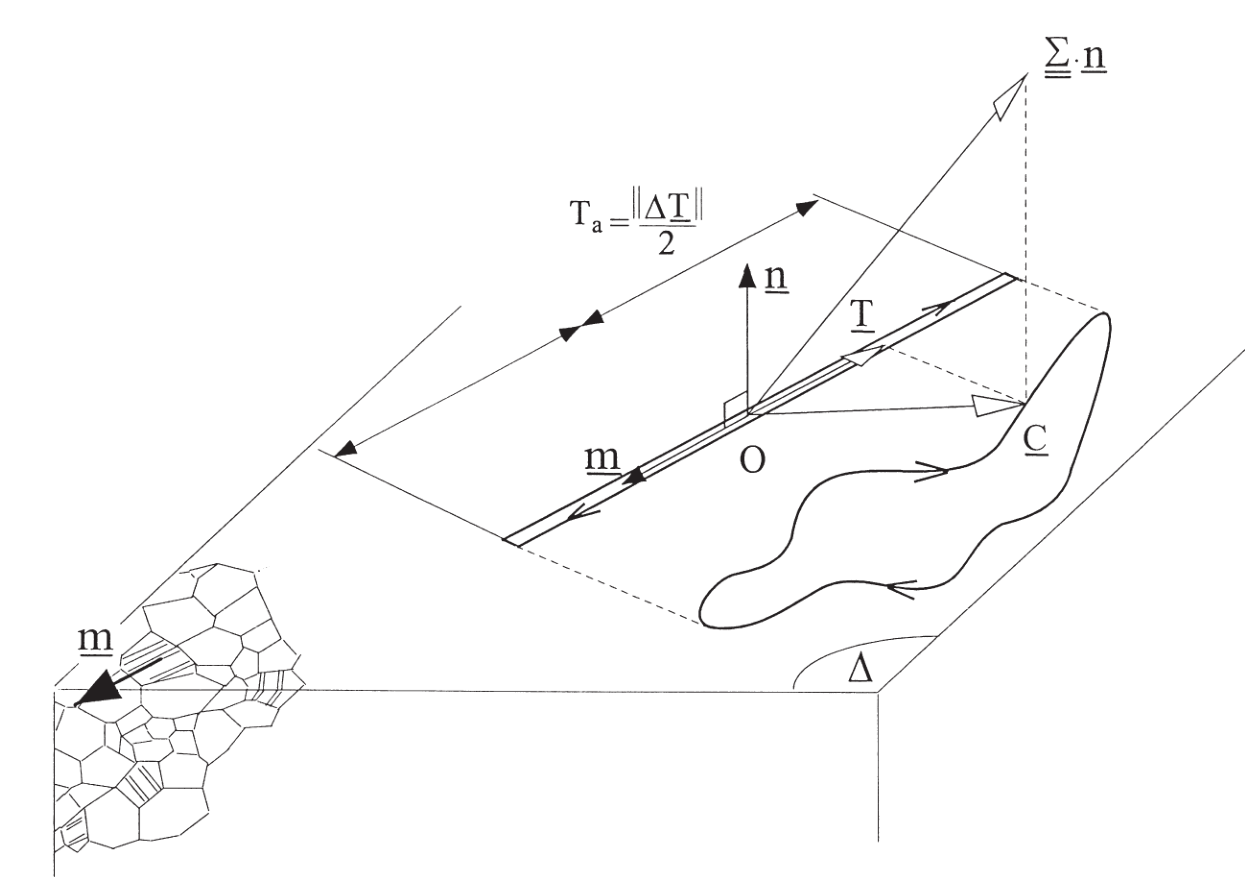
\includegraphics[width=0.8\textwidth]{figures//glid.png} 
 	\caption{Path of the macroscopic shear stress $\uline{C}$ acting on a material plane $\Delta$ and the corresponding path of the macroscopic resolved shear stress $\uline{T}$ acting on an easy glide direction.}
 	\label{glid}
 \end{figure}
\subsection{Initiation of slip in the crystal}
The plasticity criterion is determined by Schmid's law with isotropic and kinematic hardening:
\begin{equation}
f(\uline{\tau},\uline{b},\tau_y)=(\uline{\tau}-\uline{b})\cdot(\uline{\tau}-\uline{b})-\tau_y^2=0
\label{Schmid}
\end{equation}
where $\uline{b}$ is the kinematical hardening parameter back stress.

In the description of his method, the author draws heavily on the work developed by
Papadopoulos including the use of a measure of plastic deformation mesoscopic
Cumulative $T_\sigma$ associated with a particular material plane and modeling the behavior of
grain in three distinct phases (hardening, saturation and softening); he considers the cumulative mesoscopic plastic deformation $\Gamma$ as damage parameter and assumes that the initiation of a fatigue crack occurs when the latter reaches a
critical value $D = D_R = \Gamma_R$ (\figref{3phases}). 
\begin{figure}[h!]
	\centering
	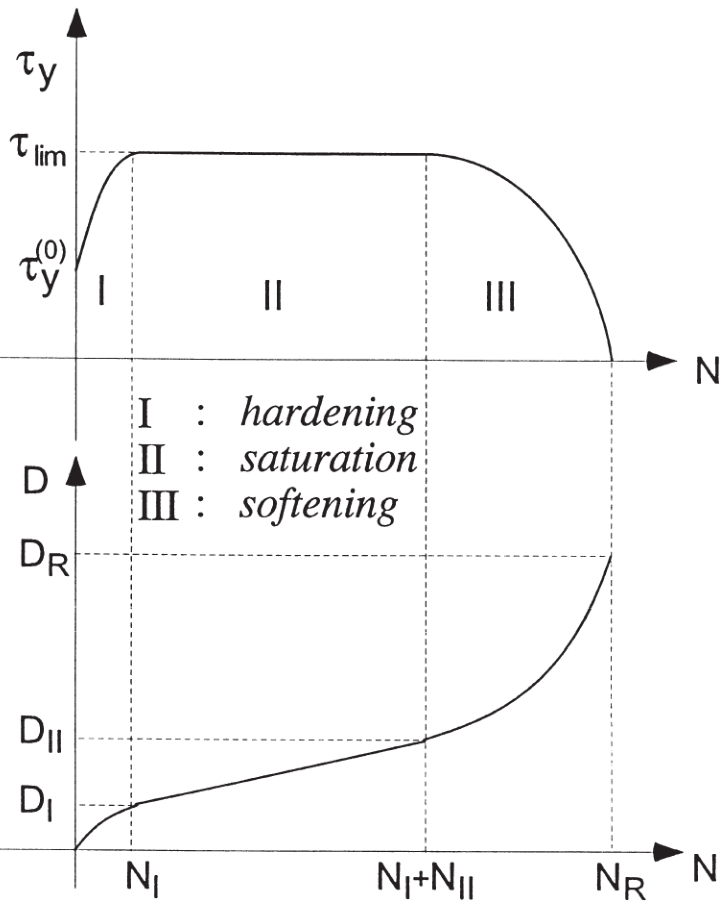
\includegraphics[width=0.5\textwidth]{figures//3phases.png} 
	\caption{Yield limit and damage evolutions in the three behavior phases (hardening, saturation and softening) when a cyclic loading	is applied.}
	\label{3phases}
\end{figure}

\subsection{Multiaxial endurance criterion}

To describe mesoscopic plasticity, Papadopoulos criterion is adopted:
\begin{equation}
\max\limits_{\theta,\varphi}(T_\sigma(\theta,\varphi))+\alpha P_{max}\leqslant \beta
	\label{papa}
\end{equation}

$T$ s is a function of the orientation of a material plane $\Delta$
through the angles $\theta$ and $\varphi$, spherical co-ordinates of the
unit normal $\uline{n}$ to the plane $\Delta$. $T_\sigma(\theta,\varphi)$ is estimated by an integration carried out
through the whole area of the plane $\Delta$:
\begin{equation}
T_\sigma(\theta,\varphi)=\sqrt{\int_{x=0}^{2\pi} T_a^2(\varphi,\theta,\psi)d\psi}
\label{Ta}
\end{equation}

$T_a$ is the amplitude of the macroscopic resolved shear
stress acting on a line of the plane $\Delta$ directed by $\uline{m}$ . This
line is determined by the angle $\psi$ from an arbitrary but
fixed axis in $\Delta$. 

The material parameters $\alpha$ and $\beta$ can be related to the
fatigue limits of two standard fatigue tests, for example
fully reversed tension-compression, $s$, and fully reversed
torsion,$t$:
\begin{equation}
\alpha=\sqrt{\pi}\frac{t-s/2}{s/3}, \beta=\sqrt{\pi}t
\end{equation}
Hereafter, the maximum value of $T_\sigma$ will be denoted as $T_\Sigma$:
\begin{equation}
T_\Sigma=\max\limits_{\theta,\varphi}(T_\sigma(\theta,\varphi))
\end{equation}


\subsection{Limit loading estimation}
The estimation of the yield limit in the saturation phase $\tau_s$ (defining the cyclic behavior of the crystal) is
carried out by the definition of a limit loading.
\begin{equation}
T_{\Sigma lim}+\alpha P_{max lim}=\beta
\end{equation}
\begin{equation}
T_{\Sigma lim}=\frac{-\alpha P_m+\beta}{\alpha+\frac{T_\Sigma}{P_a}}\cdot\frac{T_\Sigma}{P_a}
\label{Tlim}
\end{equation}
Now we need to establish $\tau_{lim}$. The corresponding actual amplitude of the shear stress,
defined as half of the longest chord of the closed curve, is denoted as $C_A$.
\begin{equation}
H=\frac{T_{\Sigma}}{C_A}=\frac{T_{\Sigma lim}}{\tau_{lim}} \, \Rightarrow \, \tau_{lim}=\frac{T_{\Sigma lim}}{H}
\label{eqH}
\end{equation}
where H constitutes a ‘phase-difference coefficient’.
It is worth mentioning that the more open the elliptic
path, the higher the coefficient H. 

\begin{figure}[h!]
	\centering
	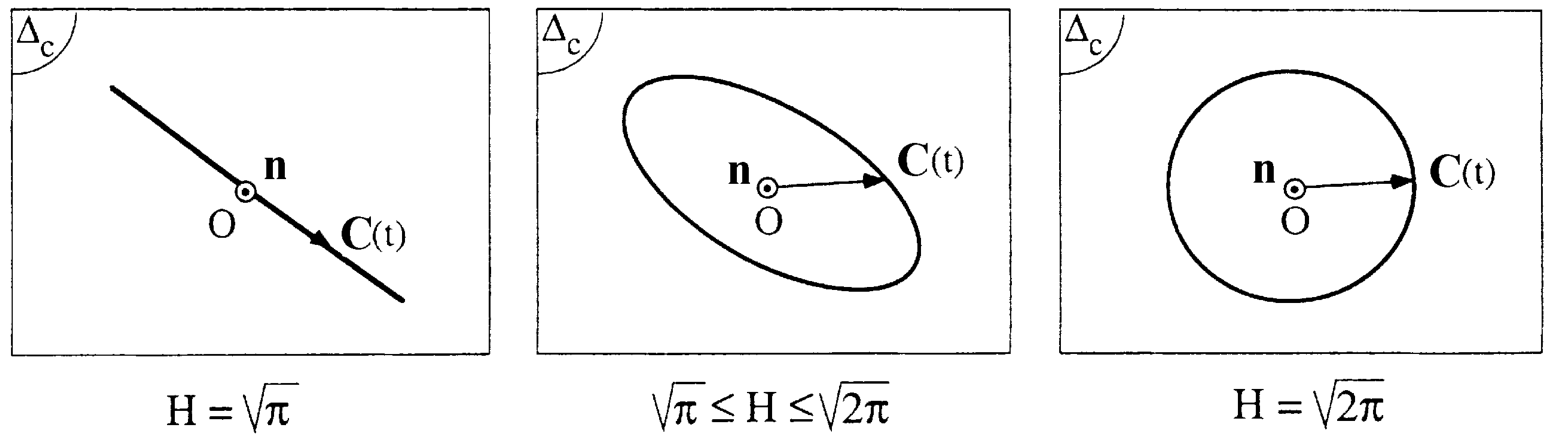
\includegraphics[width=0.9\textwidth]{figures//H.png} 
	\caption{Different paths and corresponding values of the phase-difference coefficient $H$.}
	\label{figH}
\end{figure}
For a proportional
loading, H is equal to $\sqrt{\pi}$. In the case of a particular
circular path, H reaches the maximum value $\sqrt{2\pi}$(\figref{figH}). 


\subsection{Number of cycles to failure}
Once the accumulated plastic mesostrain $\Gamma$ along the particular gliding
system reaches a critical value $\Gamma_R$, these grains are said
to be broken. An analytical expression of the number
of cycles to initiation (S–N curve) can be achieved:
\begin{equation}
\Gamma=\Gamma_R \, \Rightarrow \, N_F=pln\left(\frac{C_A}{C_A-\tau_{lim}}\right)+q\left(\frac{\tau_{lim}}{C_A-\tau_{lim}}\right)-\frac{r}{C_A}
\label{NF}
\end{equation}
where $p$, $q$ and $r$ are functions of the hardening parameters of the three phases defined above.

From Eq.\eqref{Tlim} and Eq.\eqref{eqH} we can find the yield point $\tau_s$ of the crystal in the saturation phase as a function of the amplitude $P_a$ and the mean value $P_m$ of the hydrostatic pressure, the phase difference of coefficient $H$ and two material related parameters $\alpha$ and $\beta$ :
\begin{equation}
\tau_{lim}=\tau_s=\frac{-\alpha P_m+\beta}{\alpha\frac{P_a}{C_A}+H}
\label{taus}
\end{equation}
In the last relation Eq.\eqref{NF}, the detrimental effect of out-of-phase loading is introduced through $\tau_{lim}$. As the coefficient $H$ increases, $\tau_{lim}$  decreases, therefore $N_F$ decreases which leads to more accumulated damage. The identification of the model parameters requires two endurance limits and a
single S–N curve (parameters $p$, $q$ and $r$).



\section{Variable amplitude loads}
To determine the life time in the case of multiaxial variable amplitude loads, the author performs the following steps:
\begin{flushleft}

1. Identification of the critical plane $\Delta_c$ by maximizing the standard deviation of the macroscopic resolved shear stress in different directions. The author introduces a new parameter $T_{\sigma rms}$:
\begin{equation}
T_{\sigma rms}(\theta,\varphi)=\sqrt{\int_{\psi=0}^{2\pi}T_{rms}^2(\theta,\varphi,\psi)d\psi}
	\label{srms}
\end{equation}
where $T_{rms}(\theta,\varphi,\psi)$ is the standard deviation of the macroscopic resolved shear stress.
\vspace{8pt}

2. Regarding the estimation of the phase difference coefficient H, it seems reasonable when the phase shift is not
explicitly defined (or cannot be estimated) to use the
most conservative value $\sqrt{2\pi}$.
\vspace{8pt}

3. On each direction (m) of the critical plane $\Delta_c$:
\vspace{6pt}

(a) determination of the macroscopic changes in hydrostatic pressure $P(t)$ and the macroscopic resolved shear stress $T_a(t)$;
\vspace{6pt}

(b) evaluation of the saturation point by averaging the mesoscopic resolved shear stress thresholds calculated over
the whole sequence, $\tau_{s}=(\tau_{lim})_{mean}$, $\tau_{lim}$ is calculated with Eq.\eqref{taus};
\vspace{6pt}

(c) estimation of the cumulative mesoscopic plastic strain $\Gamma$ by following the evolution of the mesoscopic yield stress $\sigma_y$  according to the three phases (hardening, saturation and softening);
\vspace{6pt}

(d) calculating the number of sequences (associated with m direction) necessary to achieve $\Gamma_R$;
\vspace{6pt}

4.  For complex multiaxial loadings, the author assumes that the hardening
and softening phases are small compared to the saturation phase\cite{Morel2000101}. In such a case, the yield limit remains constant for the whole lifetime and damage accumulation is purely linear. The analytical expression of the S–N curve(Eq.\eqref{NF}) becomes:
\begin{equation}
\Gamma=\Gamma_R \, \Rightarrow \, N_F=q\left(\frac{\tau_{lim}}{C_A-\tau_{lim}}\right)
\label{NFsimple}
\end{equation}
where$$q=\frac{c+\mu}{4}\frac{1}{l}$$

The final linear summation of individual damage from different
critical planes would then lead to damage assessment:
\begin{equation}
\sum_{i}^{}\frac{\Gamma^{(i)}}{\Gamma_R^{(i)}}=1
\label{damage}
\end{equation}

\end{flushleft}

\section{Experimental verification}
\subsection{In case of constant amplitude test }
The author \cite{FFE:FFE452} consider the example of an out-of-phase bending–torsion test on a high strength steel (30NCD16). The endurance limits of this material in reversed
bending and torsion are, respectively, $f=680 MPa$ and $t=426 MPa$.  The multiaxial sinusoidal loading is characterized by the amplitudes $\Sigma_{11a} =600 MPa$, $\Sigma_{12a} =335 MPa$ (no mean stresses)
and the phase difference $\beta_{12} =90°$.

The maximum value of $T_\sigma$ (denoted as $T_\Sigma$ ) can be deduced numerically. For this loading, we find $T_\Sigma=697 MPa$. On the critical material
plane (where $T_\Sigma$ is reached), $C_A$ is estimated to be $282 MPa$. The phase difference coefficient $H$ is
then simply deduced: $H=T_\Sigma /C_A =2.47$.

Besides noting that $P_m =0 MPa$, $P_a=200 MPa$ and $a=0.67$, $b=775 MPa$, $T_{\Sigma lim}$ is readily
computed with the help Eq.\eqref{taus}: $T_{\Sigma lim} =633 MPa$. Finally, $\tau_{lim} =T_{\Sigma lim} /H=256 MPa$. Once $p$, $q$ and $r$ have been identified from a $S–N$ curve with the least squares line method, $C_A $and $\tau_{lim}$ can
be introduced into Eq. \eqref{NF} and the number of cycles to initiation can be finally calculated, i.e.
$N_F =2×10^5$ cycles.

\subsection{In case of variable amplitude test }

 
 According to the previous endurance data and the
 definition of the generalized fatigue limit (for bending
 $\tau_{lim} =f/2$ and for torsion $\tau_{lim}=t$), one can estimate the parameter $q=20 800$.
 
 \begin{figure}[h!]
 	\centering
 	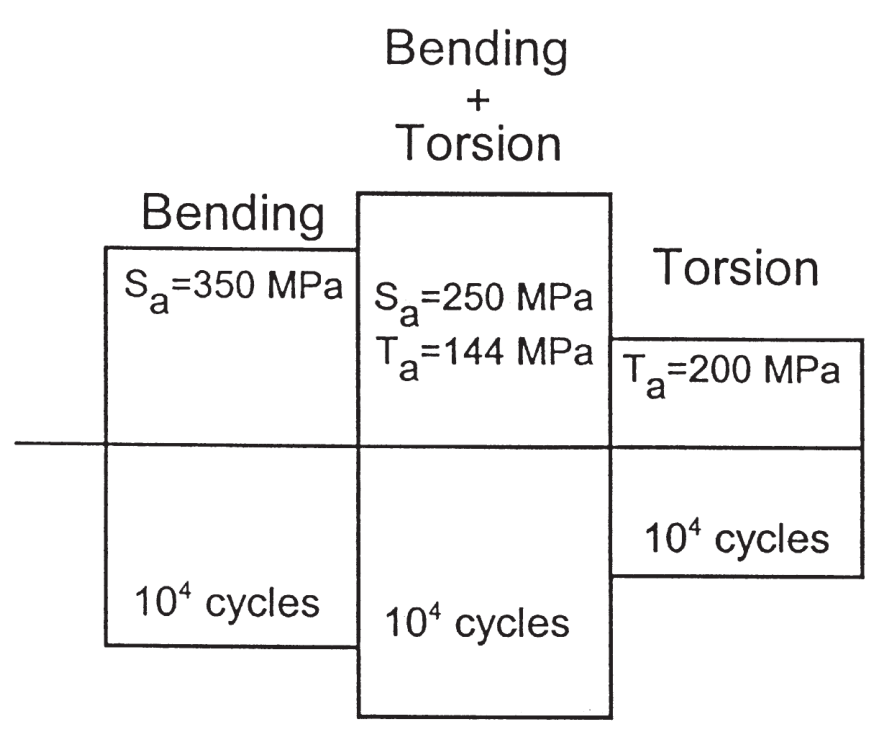
\includegraphics[width=0.6\textwidth]{figures//block.png} 
 	\caption{block sequence tests (bending/bending+torsion/torsion) performed on a mild
 		steel XC18.}
 	\label{block}
 \end{figure} 
 
 Let us consider now a block sequence composed of
 $10^4$ cycles of bending ($\Sigma_a =350 MPa$) followed by $10^4$
 cycles of combined in-phase bending–torsion ($\Sigma_a ,T_a =250 MPa, 144 MPa$)
 followed by $10^4$ cycles of torsion ($T_a =200 MPa$). This
 sequence is repeated until the initiation of a crack. The
 mean lifetime is found to be $N=1.73×10^5$ .
 
  The three generalized fatigue
  limits relative to the three blocks are estimated according
  to Eq.\eqref{taus}:
  
 $$\tau_{lim}^{bending}=155 MPa$$   $$\tau_{lim}^{torsion}=179 MPa$$  $$\tau_{lim}^{bend+tors}=157 MPa$$
  
  
 These three values and the parameter $q$ are enough to
 accumulate the damage in the three blocks using Eq.\eqref{NFsimple}:
 
 
 $$\frac{\Gamma^{(bending)}}{\Gamma_R^{(bending)}}+\frac{\Gamma^{(bend+tors)}}{\Gamma_R^{(bend+tors)}}+\frac{\Gamma^{(torsion)}}{\Gamma_R^{(torsion)}}=1$$
 
 The corresponding number of cycles to initiation is:
 $N_{prediction} <1.5×10^5$ , that is to say five successive applications of the sequence. This prediction, close to the experimental result $N=1.73×10^5$ , is a conservative one.
 
 It is important to note that if only one critical plane
 (either from bending, torsion or bending+torsion
 loading) is used for damage accumulation, one-third of
 the damage would be calculated, resulting in a nonconservative prediction.
 
\section{Discussion}
Morel's method is promising in its description aspect of limited endurance fatigue phenomenon, through the choice of the  mesoscopic plastic deformation. By using cumulative plasticity, a fatigue mechanisms occurring at the mesoscopic scale takes into account the main factors affecting the lifetime cycle fatigue (hydrostatic pressure and influence of phase shift). 

However, at the present stage, it does not completely meet the demand of a predictive tool. Indeed, it is a relatively complicated method (search critical plane $\Delta_c$ and accumulated damage in each direction in the plan); its application for multiaxial variable amplitude fatigue loads application data that are still not available (an S-N curve, two endurance limits and a particular  damage accumulation test). In addition, it is limited to soft materials. On the other hand, it is not completely free of counting method because its author uses the counting of the extrema of the evolution to get the macroscopic resolved shear stress $T(t)$ and the corresponding amplitude $P_a$ and mean values $P_m$ of the hydrostatic stress in each direction (m) in $\Delta_c$. With one purpose of calculating the limit of mesoscopic elasticity $\tau_lim$ in the saturation phase of the crystal. Again, this makes it difficult and daunting task.


\bibliographystyle{unsrt}
\bibliography{BIBbase//11}
\addcontentsline{toc}{section}{Reference }
\end{document}
%%
%% End of file `procs-template.tex'.
